% Standalone picture: the CMOS NAND as a wiring diagram in sarr.
% Compile with:  /usr/local/texlive/2024/bin/universal-darwin/pdflatex nand-wiring.tex
% Preamble below is the relevant slice of CDLM.tex (oriented WD style + \fun, \rr).

\documentclass[border=6pt]{standalone}

\usepackage{amsmath, amssymb}
\usepackage{newpxtext}
\usepackage[varg,bigdelims]{newpxmath}
\usepackage{tikz}
\usetikzlibrary{positioning, arrows.meta, decorations.markings, calc, fit, shapes}

\usepackage{booktabs}

\newcommand{\fun}[1]{\mathtt{#1}}
\newcommand{\rr}{\mathbb{R}}
\newcommand{\rv}[1]{\mathbf{#1}}
\newcommand{\ltens}{\boxtimes}
\newcommand{\inpt}[1]{#1^{-}}
\newcommand{\outp}[1]{#1^{+}}
\newcommand{\lensunit}[1][1]{\binom{#1}{#1}}
\newcommand{\sharpR}{\sharp}
\newcommand{\bang}{\mathord{!}}

\tikzset{dot/.style={circle, draw, fill=black, inner sep=0, minimum size=3pt}}
% the WD style's `ar', with its arrowhead moved to a chosen position along the path
\tikzset{arp/.style={string decoration pos=#1, ar}}

% oriented WD style (Schultz--Spivak wiring diagrams), from CDLM.tex
\tikzset{
	oriented WD/.style={
		every to/.style={out=0,in=180,draw},
    label/.style={
    	font=\everymath\expandafter{\the\everymath\scriptstyle},
      inner sep=0pt,
      node distance=2pt and -2pt},
    semithick,
    node distance=1 and 1,
    decoration={markings, mark=at position \stringdecpos with \stringdec},
    ar/.style={postaction={decorate}},
    execute at begin picture={\tikzset{
    	x=\bbx, y=\bby,
      every fit/.style={inner xsep=\bbx, inner ysep=\bby}}}
    },
    string decoration/.store in=\stringdec,
    string decoration={\arrow{stealth}},
    string decoration pos/.store in=\stringdecpos,
    string decoration pos=.5,
    bbx/.store in=\bbx,
    bbx = 1.5cm,
    bby/.store in=\bby,
    bby = 1.5ex,
    bb port sep/.store in=\bbportsep,
    bb port sep=1.5,
    bb port length/.store in=\bbportlen,
    bb port length=4pt,
    bb penetrate/.store in=\bbpenetrate,
    bb penetrate=0,
    bb min width/.store in=\bbminwidth,
    bb min width=1cm,
    bb rounded corners/.store in=\bbcorners,
    bb rounded corners=2pt,
    bb small/.style={
    	bb port sep=1, bb port length=2.5pt, bbx=.4cm, bb min width=.4cm, bby=.7ex},
    bb/.code 2 args={
    	\pgfmathsetlengthmacro{\bbheight}{\bbportsep * (max(#1,#2)+1) * \bby}
      \pgfkeysalso{draw,minimum height=\bbheight,minimum
       width=\bbminwidth,outer sep=0pt,
         rounded corners=\bbcorners,thick,
         prefix after command={\pgfextra{\let\fixname\tikzlastnode}},
         append after command={\pgfextra{\draw
            \ifnum #1=0{} \else foreach \i in {1,...,#1} {
            	($(\fixname.north west)!{\i/(#1+1)}!(\fixname.south west)$) +(-\bbportlen,0) coordinate (\fixname_in\i) -- +(\bbpenetrate,0) coordinate (\fixname_in\i')}\fi
            \ifnum #2=0{} \else foreach \i in {1,...,#2} {
            	($(\fixname.north east)!{\i/(#2+1)}!(\fixname.south east)$) +(-\bbpenetrate,0) coordinate (\fixname_out\i') -- +(\bbportlen,0) coordinate (\fixname_out\i)}\fi;
           }}}
		},
		bb name/.style={
     	append after command={
				\pgfextra{\node[anchor=north] at (\fixname.north) {#1};}
			}
		}
}

\begin{document}

\begin{minipage}{16.5cm}
\centering

% Devices at x=0 (ports top-to-bottom: gate, drain, source), reporters at x=-6.
% Vertical lanes:  a: -8.6   b: -8.0   V_dd: -3.0   V_out: -2.2   V_mid: -1.4
% The four gate levels (+1.4, -6.6, -14.6, -22.6) all miss the reporter boxes,
% so the gate wires cross the reporter column without touching it.

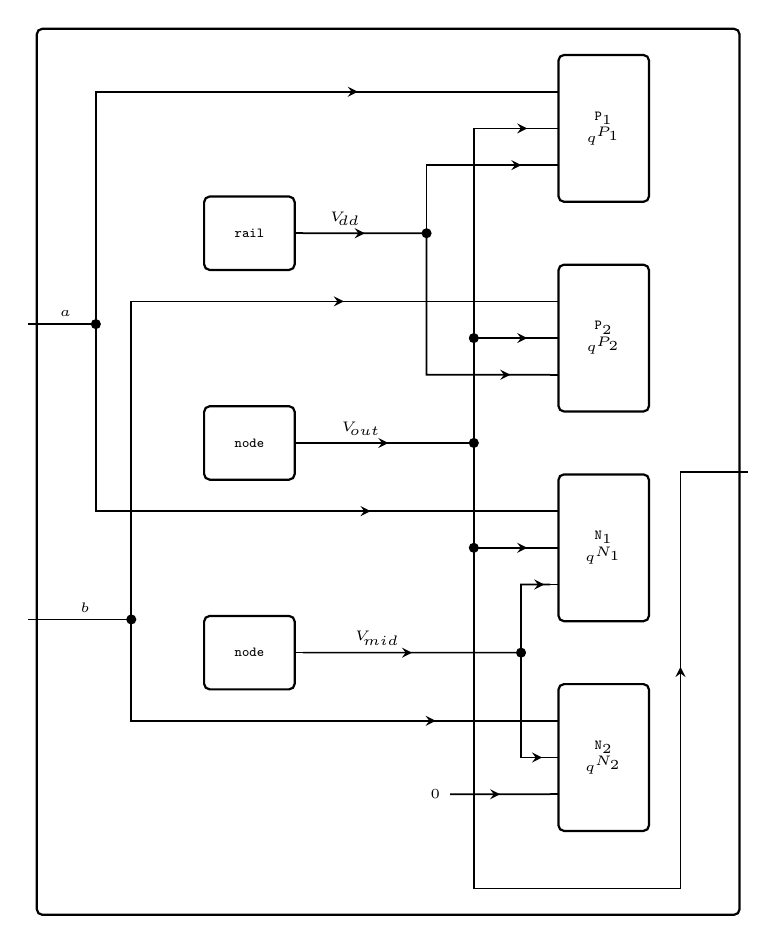
\begin{tikzpicture}[oriented WD, font=\tiny,
                    bbx=.75cm, bby=2.2ex, bb port sep=1.4,
                    bb port length=3pt, bb min width=1.15cm]

  % ---- the four devices, <R^3|R^0>
  \node[bb={3}{0}, align=center] at (0,  0) (P1) {$\fun{P}_1$\\$q^{P_1}$};
  \node[bb={3}{0}, align=center] at (0, -8) (P2) {$\fun{P}_2$\\$q^{P_2}$};
  \node[bb={3}{0}, align=center] at (0,-16) (N1) {$\fun{N}_1$\\$q^{N_1}$};
  \node[bb={3}{0}, align=center] at (0,-24) (N2) {$\fun{N}_2$\\$q^{N_2}$};

  % ---- the three voltage-reporters, <R^0|R>
  \node[bb={0}{1}] at (-6, -4) (vdd) {$\fun{rail}$};
  \node[bb={0}{1}] at (-6,-12) (out) {$\fun{node}$};
  \node[bb={0}{1}] at (-6,-20) (mid) {$\fun{node}$};

  % ---- the outer box, fit to the routing as well as the boxes
  \coordinate (tl) at (-8.6, 2.8);
  \coordinate (br) at ( 1.3,-29.0);
  \node[bb={2}{1}, fit=(tl) (br) (P1) (N2) (vdd) (mid)] (outer) {};

  % junctions on the two input lanes, at the height the outer ports sit
  \coordinate (aL) at (-8.6,0);   \coordinate (aJ) at (aL |- outer_in1);
  \coordinate (bL) at (-8.0,0);   \coordinate (bJ) at (bL |- outer_in2);

  % ================= rail -> the two PMOS sources ==============================
  \draw[ar] (vdd_out1) -- node[above=-1pt, pos=.34]{$V_{\!dd}$} (-3,-4);
  \draw[arp=.85] (-3,-4) -- (-3, -1.4) -- (P1_in3);
  \draw[arp=.85] (-3,-4) -- (-3, -9.4) -- (P2_in3);
  \node[dot] at (-3,-4) {};

  % ================= out node -> three drains, and out to the outer port =======
  % one trunk, with a dot at every T-junction so a branch never reads as a crossing
  \draw (-2.2,0) -- (-2.2,-29);
  \draw[ar] (out_out1) -- node[above=-1pt, pos=.34]{$V_{\!out}$} (-2.2,-12);
  \draw[arp=.7] (-2.2,  0) -- (P1_in2);
  \draw[arp=.7] (-2.2, -8) -- (P2_in2);
  \draw[arp=.7] (-2.2,-16) -- (N1_in2);
  \draw[arp=.62] (-2.2,-29) -- (1.3,-29) |- (outer_out1);
  \node[dot] at (-2.2,-12) {};
  \node[dot] at (-2.2, -8) {};
  \node[dot] at (-2.2,-16) {};

  % ================= mid node -> N1 source, N2 drain ===========================
  \draw[ar] (mid_out1) -- node[above=-1pt, pos=.34]{$V_{\!mid}$} (-1.4,-20);
  \draw[arp=.94] (-1.4,-20) -- (-1.4,-17.4) -- (N1_in3);
  \draw[arp=.94] (-1.4,-20) -- (-1.4,-24)   -- (N2_in2);
  \node[dot] at (-1.4,-20) {};

  % ================= outer input a -> gates of P1, N1 ==========================
  \draw (outer_in1) -- node[above=-1pt, pos=.55]{$a$} (aJ);
  \draw[arp=.72] (aJ) -- (-8.6,  1.4) -- (P1_in1);
  \draw[arp=.72] (aJ) -- (-8.6,-14.6) -- (N1_in1);
  \node[dot] at (aJ) {};

  % ================= outer input b -> gates of P2, N2 ==========================
  \draw (outer_in2) -- node[above=-1pt, pos=.55]{$b$} (bJ);
  \draw[arp=.72] (bJ) -- (-8.0, -6.6) -- (P2_in1);
  \draw[arp=.78] (bJ) -- (-8.0,-22.6) -- (N2_in1);
  \node[dot] at (bJ) {};

  % ================= ground: the constant 0, supplied by the wiring ============
  \draw[ar] (-2.6,-25.4) -- (N2_in3);
  \node[left=0pt] at (-2.6,-25.4) {$0$};

\end{tikzpicture}

\vspace{2ex}
\raggedright\footnotesize

Every wire carries $\rr$: a voltage forward, and the covector it returns --- a current --- backward.
The seven inner boxes, and the wiring that joins them:

\vspace{.6ex}
{\centering
\begin{tabular}{@{}llccl@{}}
\toprule
& type & state $\rv Q$ & reaction $\sharpR$ & potential $U$\\
\midrule
$\fun{P}_1,\fun{P}_2,\fun{N}_1,\fun{N}_2$
  & $\lensunit\to\binom{\rr^3}{\rr^0}$ & $\rr^2$
  & $\left(\begin{smallmatrix}0&1\\0&0\end{smallmatrix}\right)$
  & $\tfrac{\kappa}{2}\bigl(e_G-e_S-q_0-q_1\bigr)^2+W\bigl(q_0,\,e_D-e_S\bigr)$\\[.4ex]
$\fun{node}$ ($V_{\!out}$, $V_{\!mid}$)
  & $\lensunit\to\binom{\rr^0}{\rr}$ & $\rr$ & $1/C$ & $0$\\[.4ex]
$\fun{rail}$
  & $\lensunit\to\binom{\rr^0}{\rr}$ & $\rr$ & $0$ & $0$\\[.4ex]
the wiring
  & $\binom{\rr^3}{\rr^0}^{\ltens 4}\ltens\binom{\rr^0}{\rr}^{\ltens 3}\to\binom{\rr^2}{\rr}$
  & $\rr^0$ & --- & $0$\\
\bottomrule
\end{tabular}\par}
\vspace{1ex}

\textbf{Devices.} They report nothing and contain nothing, so $\outp f=\bang$ and $\inpt f=\bang$ and all
their content is $U$. The channel term is $W(q_0,v)=g(q_0)\,V_{\!sat}\log\cosh(v/V_{\!sat})$, so the drain
port returns $\partial_v W=g(q_0)\tanh(v/V_{\!sat})$, with $g$ a square law above threshold, mirrored for
$\fun{P}$. The reaction reads only the $q_1$-component of $dU$, and $\partial_{q_1}U=-\kappa(e_G-e_S-q_0-q_1)$
carries no $e_D$; so the gate state tracks $e_G-e_S$ with no drain back-action, for any $W$. Since $U$ sees
only differences of terminal voltages, the three port currents sum to zero.

\textbf{Reporters.} For a capacitance $C>0$, $\outp f(q)=q$, and the only covector reaching the state is the total current drawn on
the node, so the step is $q\mapsto q-\xi/C$. Taking $\sharpR=0$ freezes the state: that is the ideal
voltage source.

\textbf{The wiring} is static --- $\rv Q=\rr^0$ and $U=0$, its whole content being the two maps. $\outp f$
projects $V_{\!out}$; $\inpt f$ delivers $\fun{P}_1\mapsto(a,V_{\!out},V_{\!dd})$,
$\fun{P}_2\mapsto(b,V_{\!out},V_{\!dd})$, $\fun{N}_1\mapsto(a,V_{\!out},V_{\!mid})$,
$\fun{N}_2\mapsto(b,V_{\!mid},0)$, the last source being a constant the wiring supplies.

\textbf{The composite} is $\lensunit\to\binom{\rr^2}{\rr}$ with $\rv Q=\rr^{11}$, reaction the direct sum
of the seven reactions, and potential the sum of the four device potentials evaluated at the voltages the
wiring delivers. Nothing about the gate is written by hand: the composite potential, and with it
Kirchhoff's current law at each node, comes out of the composition.

\end{minipage}

\end{document}
